% --
% Experiments on whole dataset

\section{Experiments on whole dataset}\label{sec:exp_final}
The final experiments were performed on the whole dataset with 3500 examples per labels and are therefore used for comparison to the benchmark models shown in \rsec{prev_kws_benchmark}.
All Convolutional Neural Network (CNN) architectures were evaluated with 12 MFCC coefficients and the application of either frame-based normalization or no normalization.
A single run with 2000 epochs was performed for all experiments to save computational effort.
The evaluation on the adversarial pre-training, as described in \rsec{exp_adv}, was done for the \texttt{conv-jim} model in a separate run.
The results of the experiments are shown in \rtab{exp_final_l12}.
\begin{table}[ht!]
\small
\begin{center}
\caption{Experiment on the whole dataset with 3500 examples per label, 12 MFCC coefficients and 2000 epochs.}
\begin{tabular}{ M{3cm}  M{1.5cm}  M{2.5cm}  M{2.5cm}  M{2.5cm} }
\toprule
\multirow{2}{*}{\centering\textbf{Model Name}} & \multirow{2}{*}{\centering\textbf{Norm.}} & \multirow{2}{*}{\centering\textbf{Pre-Train}} & \multicolumn{2}{c}{\textbf{Accuracy}}\\
& & & Test set & My dataset\\
\midrule
conv-trad & 0 & - & $84.52$ & $92.00$ \\
conv-fstride & 0 & - & $79.76$ & $80.00$ \\
conv-jim & 0 & - & $87.14$ & $88.00$ \\
\midrule
conv-trad & 1 & - & $83.79$ & $88.00$ \\
conv-fstride & 1 & - & $78.71$ & $92.00$ \\
conv-jim & 1 & - & $82.36$ & $88.00$ \\
\midrule
conv-jim & 1 & adv-label-100 & $84.62$ & $92.00$ \\
\bottomrule
\label{tab:exp_final_l12}
\end{tabular}
\end{center}
\vspace{-4mm}
\end{table}
\FloatBarrier
\noindent
Note that there are some overfitting effects happening, especially showing up in the not normalized training of the \texttt{conv-trad} model in \rtab{exp_final_loss_conv-trad}.
It is therefore useful to use an early stopping technique for better generalization, that obtains the model parameters at the best performing training epoch evaluated on the validation set.
\begin{figure}[!ht]
  \centering
  \subfigure[norm0]{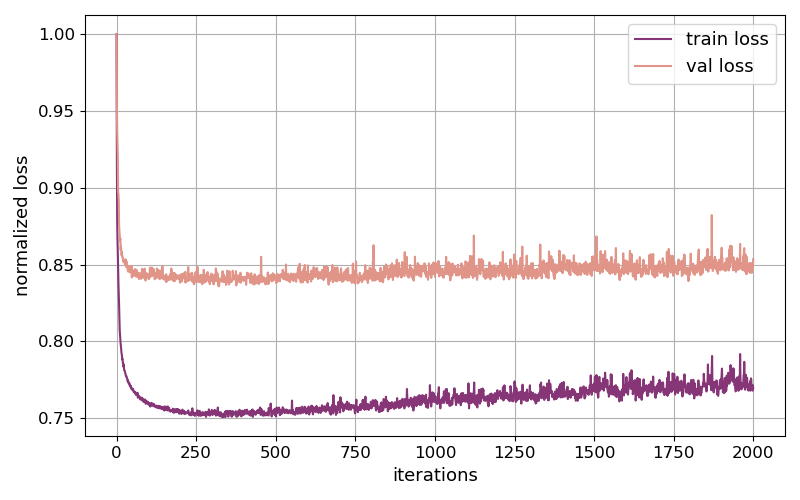
\includegraphics[width=0.45\textwidth]{./5_exp/figs/exp_final_loss_norm0_conv-trad}}
  \subfigure[norm1]{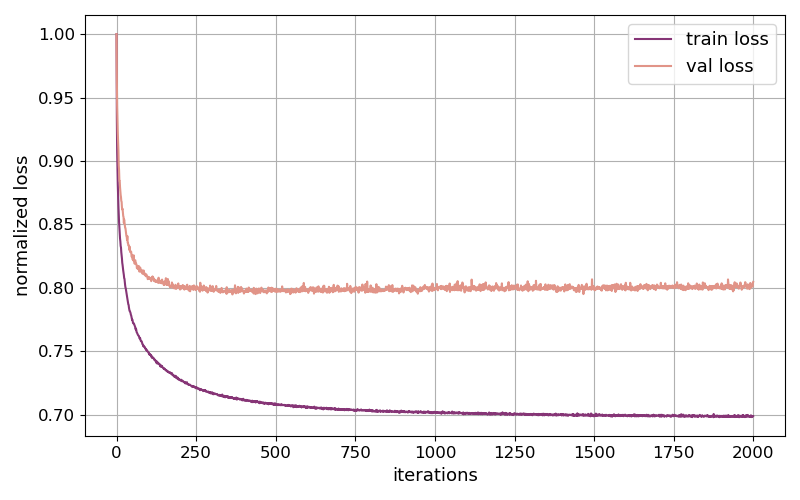
\includegraphics[width=0.45\textwidth]{./5_exp/figs/exp_final_loss_norm1_conv-trad}}
  \caption{Training loss of the \texttt{conv-trad} model showing overfitting effects on the whole dataset.}
  \label{fig:exp_final_loss_conv-trad}
\end{figure}
\FloatBarrier
\noindent
The training of models with frame-based normalization usually had less problems with overfitting compared to when using no normalization.
The accuracy performance on the validation set of all models with and without frame-based normalization is shown in \rtab{exp_final_acc}.
\begin{figure}[!ht]
  \centering
  \subfigure[norm0]{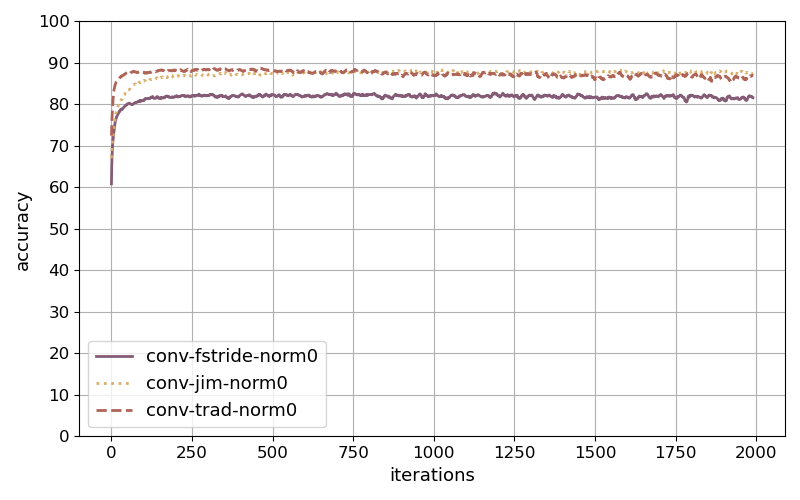
\includegraphics[width=0.45\textwidth]{./5_exp/figs/exp_final_acc_norm0}}
  \subfigure[norm1]{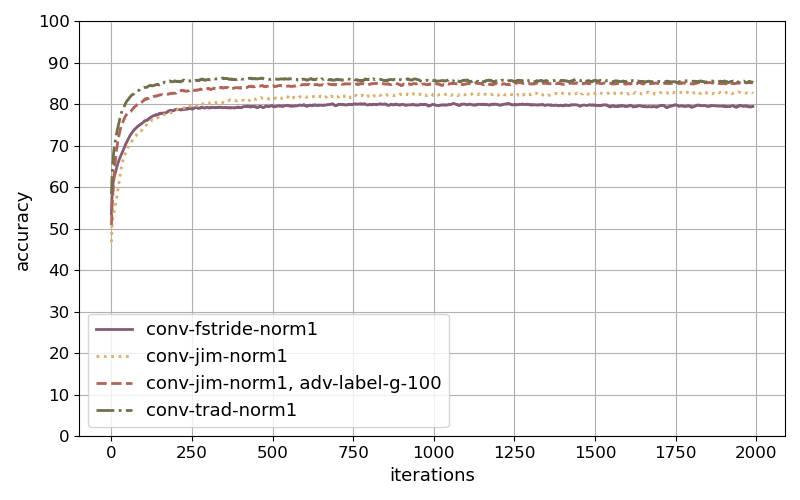
\includegraphics[width=0.45\textwidth]{./5_exp/figs/exp_final_acc_norm1}}
  \caption{Training accuracies of all models with and without frame-based normalization performed on the whole dataset, averaged over 10 epochs for better visualization.}
  \label{fig:exp_final_acc}
\end{figure}
\FloatBarrier
\noindent
Note that the the accuracy score over the epochs are not that smooth and as mentioned before it is strongly recommended to use early stopping.
That is why the \texttt{conv-trad} without frame-based normalization got a worse score than it would have achieved with early stopping.

Compared to the benchmark models, there is still a large gap to the best \texttt{conv-jim}.
With \SI{84.62}{\percent} the \texttt{conv-jim} model performs at about \SI{10}{\percent} worse than the lowest benchmark model (DS-CNN-S \cite{Zhang2017}) with \SI{94.4}{\percent}.
However it must considered that the amount of operations for the \texttt{conv-jim} model are about 6 times less than the DS-CNN-S and that not the whole audio file of \SI{1}{\second} was processed, but a shorter time interval of \SI{500}{\milli\second}.
With this in mind, the results do not look that bad.
To oberserve on where usually the classification problems are lying, a confusion matrix from the \texttt{conv-jim} model with adversarial label train on the Generator weights, is shown in \rfig{exp_final_confusion}.
\begin{figure}[!ht]
  \centering
  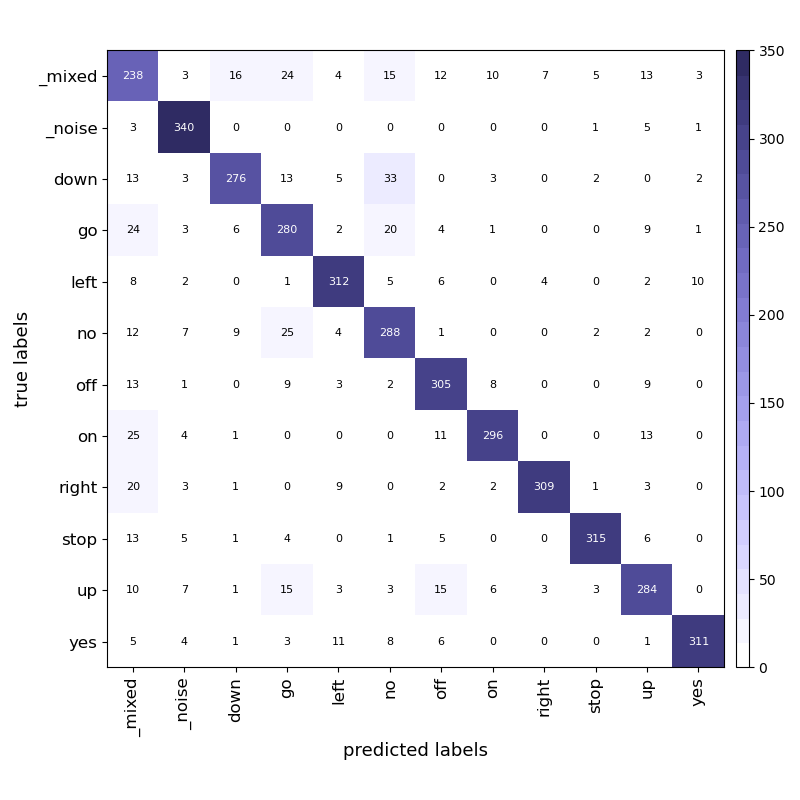
\includegraphics[width=0.45\textwidth]{./5_exp/figs/exp_final_confusion}
  \caption{Confusion matrix of the \texttt{conv-jim} model pre-trained with adversarial label train with 100 epochs on the Generator weights, and 2000 epochs of usual training, with frame-based normalization applied.}
  \label{fig:exp_final_confusion}
\end{figure}
\FloatBarrier
\noindent
From the confusion matrix it can be observed, that most classifications are done correctly and that misconceptions usually happens at similar words with the same used phonemes, like \enquote{go} and \enquote{no}.
The mixed labels also adds more difficulty in the classification task and drags the scores down.

All in all the obtained scores should be sufficient for a video game application.